\documentclass[11pt]{article}
\usepackage{graphicx}
\usepackage{amssymb}
%\usepackage[nomarkers]{endfloat}
\usepackage{natbib}
\usepackage{setspace}
\usepackage{wasysym}
\usepackage{wrapfig}
\pagestyle{empty}
\textwidth = 7 in
\textheight = 9 in
\oddsidemargin = -0.5 in
\evensidemargin = -0.5 in
\topmargin = 0.0 in
\headheight = 0.0 in
\headsep = 0.0 in
\parskip = 0.1in
\parindent = 0in
\renewcommand{\Pr}{\mathbb{P}}
\usepackage{paralist}
\usepackage{url}
\newcommand{\href}[2]{\url{#2}}
\usepackage{tikz}
  \usetikzlibrary{shapes.geometric}
  \usetikzlibrary{arrows.meta,arrows}
  \usetikzlibrary{positioning,automata}
\tikzstyle{line}=[draw]
\usepackage{hyperref}
\hypersetup{backref,   linkcolor=blue, citecolor=red, colorlinks=true, hyperindex=true}
\begin{document}
\resizebox{\textwidth}{!}{
    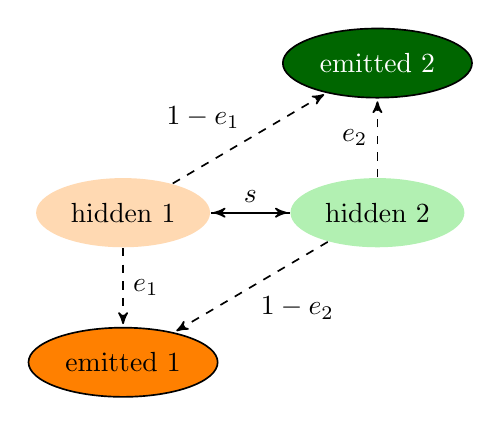
\begin{tikzpicture}[->,>=stealth',shorten >=1pt,auto,semithick,every state/.style={fill=red,draw=none,text=black,shape=ellipse}]
\node[state, fill=orange!30!,text=black]  (h1) {hidden 1};
\node[state, fill=black!20!green!30!,text=black] (h2) [right=of h1] {hidden 2};
\node[state, fill=orange,text=black, draw=black] (v1) [below=of h1] {emitted 1};
\node[state, fill=black!60!green,text=white, draw=black] (v2) [above=of h2] {emitted 2};
\path (h1) edge node {${s}$} (h2) ;
\path (h2) edge node {} (h1) ;
\path (h1) edge [style=dashed] node [pos=.5] {$e_{1}$} (v1) ;
\path (h1) edge [style=dashed] node [pos=.5] {{$1-e_{1}$}} (v2) ;
\path (h2) edge [style=dashed] node [pos=.5] {$1- e_{2}$} (v1) ;
\path (h2) edge [style=dashed] node [pos=.5] {{$e_{2}$}} (v2) ;
\end{tikzpicture}

}

\end{document}